\documentclass[spanish,11pt,letterpaper,oneside]{memoir}
% Configuración del idioma español
\usepackage[T1]{fontenc}
\usepackage[utf8]{inputenc}
\usepackage[spanish]{babel}
\usepackage{graphicx}
\usepackage{wrapfig}
\usepackage{amsmath}
\usepackage[spanish,onelanguage,ruled,vlined]{algorithm2e}
\usepackage{csquotes}
% Configuración de las citas bibliográficas (puedes cambiarlo según tu preferencia)
%\usepackage[backend=biber,style=ieee]{biblatex}


% Personalización de los nombres de los capítulos y otros elementos
\renewcommand{\partname}{Parte}
\renewcommand{\chaptername}{Capítulo}
\renewcommand{\bibname}{Bibliografía}
\renewcommand{\contentsname}{Tabla de contenidos}
\renewcommand{\listfigurename}{Lista de figuras}
\renewcommand{\listtablename}{Lista de tablas}

\begin{document}
\frontmatter
% Portada
\begin{titlingpage}
  \begin{center}
  	{
\includegraphics[width=0.35\linewidth]{Sem_1/figuras/ulaLogo}\par}
  	\vspace{1cm}
	\begin{Large}
		Universidad de los Andes \\
		Facultad de Ciencias \\ 
		Departamento de Física \\ 
		Laboratorio de Física Aplicada\par
	\end{Large}
	\vspace{0.7cm}
	\textbf{{\Large Búsqueda de agrupaciones en data proveniente de electrocardiogramas (ECG), mediante el Análisis de Componentes Principales (PCA) y el uso de Redes Neuronales.}}\par
	\vspace{0.5cm}
	{\itshape\large Trabajo especial de grado.}\par
	\vspace{0.5cm}
	{\large\textbf{Br. Abrahan David Quintero Teran}}\par
   	\vspace{0.5cm}
    {\large Tutor: Prof. Juan Villegas}\par
    \vspace{0.5cm}
    \begin{flushright}
    	{\large Jurados: \par
    	Prof. Marcos Rodríguez \par
    	Prof. John Ferreira \par}
    \end{flushright}
    {\large\textbf{Mérida -- Venezuela}} \par
    {\large 2024} % Deja esto vacío para eliminar la fecha de la portada
  \end{center}
\end{titlingpage}

% Abstract en español
\begin{abstract}
  Este es el resumen de mi tesis.
\end{abstract}


\newpage
% Abstract en inglés (opcional)
% \begin{otherlanguage}{english}
% \begin{abstract}
% This is the abstract of your thesis in English.
% \end{abstract}
% \end{otherlanguage}

\tableofcontents*
\mainmatter


%\part{Primer Seminario}
\pagestyle{empty}{\huge\textbf{Introducción}}
\chapter{El problema}
	El electrocardiograma (ECG) es una técnica no invasiva que permite registrar y medir las señales eléctricas generadas por el corazón. Consiste en la captación de la variación temporal del potencial bioeléctrico durante cada ciclo cardíaco, utilizando electrodos colocados en la superficie cutánea del paciente que registran dicha actividad eléctrica y producen un gráfico que muestra el ritmo y la fuerza de los latidos del corazón, este produce un patrón muy específico, y cualquier anomalía puede indicar un problema cardíaco \cite{ZHANG2021113}. El análisis del ECG proporciona datos sobre el sistema cardiovascular, en particular, el corazón, lo que permite detectar diversas enfermedades que pueden afectar su funcionamiento óptimo. Estas enfermedades incluyen arritmias cardíacas, obstrucción de arterias, insuficiencia cardíaca y ataques al corazón \cite{MedlineECG}. \\ Según la organización mundial de la salud \cite{Who}, las enfermedades cardiovasculares (ECV) son las principal causa de muerte en hombres y mujeres en el mundo, con alrededor de 17,9 millones de personas que mueren al año a causa de estas. Entre los numerosos factores que llevan a esta consecuencia, se encuentran los errores provenientes de la interpretación manual de los electrocardiogramas (ECGs), por lo general, los médicos emplean características heurísticas diseñadas manualmente o utilizan arquitecturas de aprendizaje de características superficiales, esto puede generar como consecuencia, variabilidad entre los diagnósticos de los observadores e identificación de anomalías incorrectas que pueden llevar a ocasionar diagnósticos imprecisos y en consecuencia, tratamientos inadecuados. Además estos métodos manuales que utilizan arquitecturas de aprendizaje de características superficiales, descartan información relevante del ECG inmersa dentro de características que no son superficiales, lo que provee una baja exactitud en el diagnostico a partir de las señales por lo que siempre será necesario de la supervisión de un experto con el fin de corregir estos errores, además algunas enfermedades cardíacas, como la enfermedad de las arterias coronarias en etapa temprana, pueden no ser detectables en un ECG, también se debe resaltar, que el ECG se puede ver afectado por factores externos, como el movimiento del paciente, las interferencias electromagnéticas, la incorrecta colocación de los electrodos, estados ansiosos de los pacientes al momento de aplicarles el examen o el uso de medicamentos.

\section{Justificación}
	La interpretación manual de los ECGs está sujeta a errores humanos por fatiga, sesgos o variabilidad interobservador, lo que puede generar diagnósticos incorrectos y por ende, tratamientos inadecuados. Además, el ECG contiene información oculta (como edad, sexo o incluso identidad del paciente) que el ojo humano no puede cuantificar o identificar sistemáticamente. Aunque existen herramientas digitales para análisis de ECG, la mayoría se limitan a detectar arritmias básicas y no aprovechan el potencial que tiene el ECG como biomarcador  para extraer caracteristicas clínicas no evidentes e incluso llegar a identificar a cada paciente, es por esto que resulta importante desarrollar herramientas que puedan procesar los ECG para reducir o eliminar la presencia de ruidos e interferencias y así minimizar los errores manuales mediante algoritmos robustos y adaptables, descubriendo patrones clínicos con modelos profundos y hasta siendo capaz de identificar pacientes usando el ECG como firma biológica
	
	%Ante la necesidad de reducir los errores provenientes de la interpretación manual de los ECGs que junto con la presencia de ruidos e interferencias en las señales que complican aún más el análisis del ECG, surge la necesidad de desarrollar herramientas reduzcan estos errores. Por lo que el desarrollo de técnicas que ayuden a minimizar la presencia de ruidos e interferencias en los ECG, sin afectar la morfología real del ECG, pueden resultar muy útiles para la posterior identificación de patrones específicos y clasificación precisa en grupos de pacientes que, siguen siendo desafíos importantes, ya que los métodos tradicionales de análisis de ECGs a menudo no son lo suficientemente robustos para manejar estas complejidades de manera eficiente. Es por esto que el desarrollo de nuevas tecnologias que favorezcan la debida identificación de caracteristicas clínicas, como lo pueden ser el estado de salud, mientras se usan métodos robustos y adaptables como el aprendizaje automático, que son capaces de por ejemplo, de reducir dimensiones en la data para manejar de manera eficiente los recursos computaciones, pudieran tener un impacto positivo en posteriores estudios donde se desarrollen herramientas que utilicen principalmente estas caracteristicas clínicas, para el análisis de ECGs.
 

\section{Objetivos}
\subsection{Objetivo General}
Analizar los datos provenientes de electrocardiogramas mediante la aplicación de análisis de componentes principales (PCA) y redes neuronales, con el objetivo de identificar agrupaciones en dicha data.
\subsection{Objetivos específicos}
\begin{enumerate}
	\item Implementar técnicas avanzadas de filtrado y eliminación de artefactos para obtener señales de electrocardiogramas más limpias.
	\item Desarrollar un marco metodológico solido que combine el análisis de componentes principales (PCA) y redes neuronales perceptrónicas para la identificación de grupos de datos.
	\item Evaluar el rendimiento de los modelos propuestos utilizando los datasets de electrocardiogramas de las bases de datos de Physionet.
\end{enumerate}



\chapter{Marco Teórico}

\section{Antecedentes}
	
La electrocardiografía sigue siendo uno de los bastiones en lo que se basa la cardiología moderna para el diagnostico de cardiopatías, el electrocardiograma (ECG) suele ser el primer examen que se le realiza a cada paciente cuando se examina a profundidad, ya que es capaz de arrojar información importante del funcionamiento del sistema circulatorio y podría rociar indicios de problemas que pudieran estar pasando en otros sistemas importantes del cuerpo humano. La ciencia siempre ha acompañado la innovación y creación de nuevas tecnologías y la física, como baluarte entre las ciencias naturales, se ha interesado en contribuir en el mejoramiento de estas tecnologías, aportando eficacia y rendimiento desde ángulos no antes vistos. Esto ha conducido a investigar referentes, que permiten ampliar el panorama científico que hay detrás de un ECG. 
Ahora se presentan una serie de investigaciones que continúan con esta linea de investigación, que consiste en aplicar métodos computaciones a la salud, creciente interés que ha incrementado desde finales del siglo pasado. \\
	
\subsection{A Real-Time QRS Detection Algorithm \cite{PanTompkins85}}
\textbf{Autores:} Pan, Jiapu; Tompkins, Willis J. 

\textbf{Publicación:} IEEE Transactions on Biomedical Engineering

\textbf{DOI:} 10.1109/TBME.1985.325532

\textbf{Resumen:} Pan y Tompkins presentan el primer algoritmo para detectar en tiempo real el complejo QRS de las señales de ECG. Este algoritmo es capaz de reconocer con fiabilidad los complejos QRS basándose en análisis digitales de la pendiente, la amplitud y la anchura. Además, se plantan las bases de filtrado que se le debe hacer a una señal de ECG para reducir las falsas detecciones causadas por los distintos tipos de interferencias presentes en las señales de ECG, aumentando así la sensibilidad de la detección.

\textbf{Metodología:} 
\begin{enumerate}
	\item \textbf{Filtro pasa-banda:} Como primer paso, se aplica un filtro pasa-banda, a la señal del ECG, para incrementar la relación señal-ruido, se sugiere un filtro con un ancho de banda de 5-15 Hz para maximizar el QRS y también reducir el ruido producido por el movimiento de los músculos y el desplazamiento de la linea base.
	\item \textbf{Filtro derivativo:} Se aplica un filtro derivativo para proveer información acerca de la pendiente del QRS.
	\item \textbf{Cuadratura e integración:} La señal filtrada se eleva al cuadrado para realzar los picos dominantes (QRS) y reducir la posibilidad de reconocer erróneamente una onda T como pico R. A continuación, se aplica un filtro de media móvil para proporcionar información sobre la duración del complejo QRS.
\end{enumerate}
	
\textbf{Hallazgos clave:}
\begin{itemize}
	\item La serie de filtros aplicados resaltan el contenido frecuencial de la rápida despolarización cardíaca y elimina el ruido de fondo.
	\item Identifica los QRS en tiempo real con un costo computacional bajo.
	\item Se reportó que el porcentaje de acierto del QRS fue de 99.3\%
\end{itemize}

%Esto está comentado porque no me parecio apropiado poner este articulo entre los antecedentes
%\subsection{Adaptative estimation of QRS complex wave features of ECG signal by the Hermite model \cite{Laguna97}}
%\textbf{Autores:} Laguna, P.; Jané, R.; Olmos, S.; Thakor N.V.; Rix, H.; Caminal, P.
%
%\textbf{Publicación:} PubMed \textbf{DOI:} 10.1007/BF02367023
%
%\textbf{Resumen:} En este estudio se presenta un sistema de estimación adaptativa del modelo de Hermite (AHMES) para la estimación en línea, latido a latido de las caracteristicas que describen el QRS con el modelo de Hermite. Este sistema permite una extracción eficiente de parámetros en tiempo real para la clasificación y compresión de datos.
%
%\textbf{Metodología:}
%
%\textbf{Hallazgos clave:}

\subsection{A Wavelet-Based ECG Delineator: Evaluation on Standard Databases \cite{Martinez04}}
\textbf{Autores:} Martínez, J. P.; Almeida, R.; Olmos, S.; Rocha, A. P., Laguna, P.

\textbf{Publicación:} IEEE Transactions on Biomedical Engineering
\textbf{DOI:} 10.1109/TBME.2003.821031

\textbf{Resumen:} En este artículo, desarrollan y evalúan un robusto sistema de delineación de ECG de una sola derivación basado en las transformada de ondícula (WT, por sus siglas en inglés). Primeramente, detectan los complejos QRS para luego delimitar cada QRS, detectando e identificando los picos de las ondas individuales, así como también, los inicios y finales de cada complejo QRS. Finalmente, se realiza la determinación de los picos, inicios y finales de las ondas P y T. Posteriormente, se evalúa este algoritmo en varias bases de datos anotadas manualmente, como MIT-BIH Arritmia \cite{arritmiadb}, QT \cite{qtdb}, ST-T Europea \cite{st-tdb} y otras bases de datos, desarrolladas para propósitos de validación.

\textbf{Metodología:} 
\begin{itemize}
	\item Usando la transformada de ondícula discreta (DWT, por sus siglas en inglés), pueden detectar las ondas presentes en un ECG que están compuestas por pendientes y máximos (o mínimos) locales a diferentes escalas, ocurriendo a diferentes instantes de tiempo dentro del ciclo cardíaco.
	\item Primero, se detecta el complejo QRS para luego detectar e identificar las ondas individuales presentes en este; y posteriormente, determinar los limites del complejo QRS.
	\item Por ultimo se detectan y delimitan las ondas T y P respectivamente.
\end{itemize}

\textbf{Hallazgos clave:}
\begin{itemize}
	\item El algoritmo propuesto por Martínez \textit{et al.} es capaz de identificar y ubicar en función del tiempo las ondas individuales de cada latido.
	\item Este método es lo suficiente robusto como para permitir la aplicación directa de este sobre señales de ECG sin previo filtrado.
	\item Obtuvieron un porcentaje de detección superior al $99.86\%$ para la base de datos MIT-BIH Arritmia \cite{arritmiadb} y del $99.88\%$ para la base de datos QT \cite{qtdb}.
\end{itemize}

\subsection{Feature extraction for heartbeat classification using independent component analysis and matching pursuits \cite{Herrero05}}

\textbf{Autores:}Herrero, G.G.; Gotchev, A.; Christov, I.; Egiazarian, K.

\textbf{Publicación:} IEEE
\textbf{DOI:} 10.1109/ICASSP.2005.1416111

\textbf{Resumen:} En esta investigación, se presenta un método basado en el algoritmo de búsqueda de coincidencias para la extracción de caracteristicas de tiempo-frecuencia que pueden ser usadas para la clasificación de varios tipos de latidos anormales. Luego de esto, investigan sobre la usabilidad del análisis de componentes independientes (ICA, por sus siglas en inglés) para extraer caracteristicas espaciales de grabaciones de electrocardiogramas de varias derivaciones. El rendimiento de estos diferentes conjuntos de caracteristicas es evaluado usando las grabaciones de la base de datos MIT-BIH Arritmia \cite{arritmiadb}.

\textbf{Metodología:} 
\begin{itemize}
	\item Habiendo detectado los latidos anotados en la base de datos y usando las dos derivaciones presentes en dicha base de datos, el bloque de ICA estima para cada latido, una matriz de proyección que minimiza la dependencia estadística entre las dimensiones proyectadas.
	\item Las componentes de la matriz antes mencionadas, son usadas como caracteristicas para la etapa de clasificación.
	\item La extracción de caracteristicas de tiempo-frecuencia proyecta cada latido en conjuntos diferentes de paquetes de onda que se seleccionan para que coincidan con las estructuras caracteristicas de los distintos tipos de latidos que se intentan clasifican.
	\item Por ultimo, las caracteristicas de tiempo-frecuencia e ICA se clasifican mediante redes neuronales.
\end{itemize}

\textbf{Hallazgos clave:} 
\begin{itemize}
	\item Introducen ICA como extractor de caracteristicas para el procesamientos de los ECGs.
	\item El rendimiento del sistema tuvo una precisión superior al $95\%$ en la clasificación de 5 tipos de latidos anormales.
	\item La potencia computacional requerida para el sistema propuesto es bastante alta durante el entrenamiento del extractor de caracteristicas
\end{itemize}

\subsection{Sistema de adquisición multicanal y análisis de la señal electrocardiográfica de alta resolución aplicado a pacientes chagásicos \cite{Dugarte11}}
\textbf{Autores:} Dugarte, N.; Cuadros, J.; Medina, R.; Rojas, R.; Jugo, D. Nuñez, T.

\textbf{Publicación:} Conferencia: XI Congreso Internacional de Métodos Numéricos en Ingeniería y Ciencias Aplicadas
%\textbf{DOI:} no tiene doi porque es una exposicion de una conferencia

\textbf{Resumen:} En este trabajo, se reporta el desarrollo de un sistema integral para adquisición y posterior análisis de la señal electrocardiográfica de alta resolución (ECGAR) de pacientes chagásicos, en el cual utilizan maquinas de soporte vectorial de mínimos cuadrados (LSSVM, por sus siglas en inglés) para determinar el inicio del complejo QRS y el final de la onda T, para estimar los intervalos QT y QT corregido (\textit{QTc}) y comparan su efectividad usando algoritmos de procesamiento implementados en la aplicación Cardiosoft \cite{cardiosoft}. 

\textbf{Metodología:}
\begin{itemize}
	\item Se les realizó un registro ECGAR a 20 pacientes chagásicos, excluyendo pacientes con otras patologías y 20 pacientes de control.
	\item Utilizan LSSVM para determinar el inicio del complejo QRS y el final de la onda T, entrenadas en base a atributos extraídos de la señal preprocesada y de señales obtenidas mediante descomposiciones con Wavelets.
	\item Se estiman tanto el intervalo QT y el QT corregido (\textit{QTc}) con el uso de las técnicas antes mencionadas.
\end{itemize}

\textbf{Hallazgos clave:}
\begin{itemize}
	\item Estudian la efectividad de este análisis en el reconocimiento de pacientes chagásicos al procesar, 20 pacientes chagásicos y 20 sujetos de control.
	\item Los resultados muestran diferencias estilísticamente significativas entre ambos grupos.
	\item Validan los algoritmos de procesamiento implementados utilizando como referencia una aplicación denominada Cardiosoft \cite{cardiosoft}.
\end{itemize}

\subsection{A comparative study of DWT, CWT and DCT transformations in ECG arrhythmias classification \cite{Khorrami10}.}
\textbf{Autores:} Khorrami, H.; Moavenian M.
 
\textbf{Publicación:} Expert Systems with Applications
\textbf{DOI:} 10.1016/j.eswa.2010.02.033

\textbf{Resumen:} En este estudio, se sugiere y comparan el uso de transformadas ondículas discretas (CWT, por sus siglas en inglés), transformadas ondículas discretas (DWT) y transformada discreta del coseno (DCT, por sus siglas en inglés), que ya están en uso, con el fin de mejorar la capacidad de dos clasificadores de patrones en clasificación de arritmias en señales de ECG. Se utilizan como clasificadores, redes neuronales perceptrónicas y máquinas de soporte vectorial. Las señales de ECG usadas son tomadas de la base de datos Arritmia del MIT-BIH que son usadas para clasificar cuatro diferentes tipos de arritmias. 

\textbf{Metodología:}
\begin{itemize}
	\item Las técnicas de extracción de caracteristicas CWT, DWT y DCT son aplicadas separadamente a la base de datos antes de su clasificación.
	\item Utilizan estas características extraídas para clasificar los tipos de arritmia de cada señal de ECG, usando redes neuronales perceptrónicas (NN, por sus siglas en inglés) y máquinas de soporte vectorial (SVM, por sus siglas en inglés).
	\item Comparan el rendimiento del entrenamiento, el rendimiento de las pruebas y el tiempo de entrenamiento de cada clasificador. 
\end{itemize}

\textbf{Hallazgos clave:}
\begin{itemize}
	\item Los resultados muestran que el mejor método de extracción de caracteristicas dependerá del valor sustancial que se considere para el tiempo de entrenamiento y rendimiento en el entrenamiento y las pruebas.
	\item El rendimiento de las pruebas, usando sólo la derivación II de la señal de ECG usada muestra superioridad sobre las SVM.
	\item El modelo que utiliza como extractor de caracteristicas las DWT y una NN como clasificador es el que tiene mejor rendimiento tanto en entrenamiento y pruebas, como en tiempo de entrenamiento.
\end{itemize}

\subsection{Comparison of FCM, PCA and WT techniques for classification ECG arrhythmias using artificial neural network \cite{Ceylan07}.}

\textbf{Autores:} Ceylan, R.; Özbay, Y.

\textbf{Publicación:} Expert Systems with Applications.
\textbf{DOI:} 10.1016/j.eswa.2006.05.014

\textbf{Resumen:} Este articulo presenta un estudio comparativo de la eficacia en la clasificación de señales ECG usando 4 tipos de estructuras que incluyen poderosas técnicas de reducción de dimensionalidad, como lo son PCA, WT y agrupamiento c-medios difuso (FCM, por sus siglas en inglés); también usan redes neuronales perceptrónicas (NN) para clasificar tipos de arritmias, usando MIT-BIH Arritmia \cite{arritmiadb}, estas son entrenadas para clasificar 10 diferentes tipos de arritmias. 

\textbf{Metodología:}
\begin{itemize}
	\item Utilizando PCA y WT para reducción de caracteristicas en adición de FCM; y NN para clasificar los tipos de arritmia en las señales de ECG, comparan el desempeño de 4 tipos de estructuras propuestas, FCM-NN, PCA-NN, FCM-PCA-NN y WT-NN.
	\item Prueban cada uno de los modelos propuestos con las señales de ECG tomadas de MIT-BIH Arritmia\cite{arritmiadb}.
\end{itemize}

\textbf{Hallazgos clave:}
\begin{itemize}
	\item Proponen como nuevo método de clasificación, la estructura FCM-PCA-NN.
	\item Las pruebas realizadas sugieren que la estructura FCM-PCA-NN puede generalizar mejor que PCA-NN y mucho más rápido de las demás estructuras propuestas.
	\item Si bien, la estructura FCM-PCA-NN presenta el menor error ($5.05\times10^{-9} \% $) al clasificar los tipos de arritmias, es importante señalar que el modelo PCA-NN no se queda atrás en desempeño, teniendo un error de ($4.98\times10^{-9} \%$). Esta mínima diferencia sugiere que ambas arquitecturas, podrían considerarse alternativas viables.
\end{itemize}

\subsection{Baseline wander removal of ECG signals using Hilbert vibration decomposition \cite{Sharma15}.}

\textbf{Autores:}Sharma, H.; Sharma, K. K.

\textbf{Publicación:} Electronics Letters.
\textbf{DOI:} 10.1016/j.eswa.2010.02.033

\textbf{Resumen:} En este estudio, se propone una técnica para remover el desplazamiento de la línea base (BW, por sus siglas en inglés) de las señales de ECG utilizando la descomposición vibracional de Hilbert (HVD, por sus siglas en inglés). Se plantea que la primera componente (la componente de más alta energía) usando HVD en la señal de ECG corresponde al BW de la señal. La técnica propuesta es comparada con otro método basado en descomposición modal empírica (EMD, por sus siglas en inglés) y matemática morfológica, en términos de criterios de correlación y relación señal-ruido. 

\textbf{Metodología:}
\begin{itemize}
	\item Para lograr remover el desplazamiento de la línea base, primero se descompone la señal ECG usando HVD en sus diversas componentes, siendo la primera de estas, la de más alta energía y por ende, la correspondiente al BW.
	\item Luego corrigen la señal de ECG, sustrayendo la primera componente de la HVD de la señal original.
	\item Para evaluar el desempeño de la técnica propuesta, se usan las señales electrocardiográficas de MIT-BIH Arritmia \cite{arritmiadb} y le introducen un BW artificial obtenido de un filtrado paso bajo de señales aleatoriamente generadas.
\end{itemize}

\textbf{Hallazgos clave:}
\begin{itemize}
	\item La técnica propuesta en este articulo, tiene un mejor desempeño que la aproximación basada en EMD para remover el BW.
	\item También se observa que la HVD es computacionalmente eficiente. 
	\item El método propuesto es capaz de desempeñarse mejor bajo condiciones de severa distorsión de la linea base sin afectar la morfología real del ECG.
\end{itemize}

\subsection{Heart failure classification using deep learning to extract spatiotemporal features from ECG \cite{Zhang24}}
\textbf{Autores:} Zhang, C.; Yuan, Lu.; Tang, F.; Cai, H.; Qian, Y.; Wang, C.

\textbf{Publicación:} BMC Medical Informatics and Decision Making.
\textbf{DOI:} 10.1186/s12911-024-02415-4

\textbf{Resumen:} La insuficiencia cardíaca es un síndrome con complejas manifestaciones clínicas. Debido al creciente envejecimiento de la población, la insuficiencia cardíaca se ha convertido en uno de los mayores problemas alrededor del mundo. Este estudio, se usa la base de datos pública MIMIC-III para extraer las caracteristicas temporales y espaciales de las señales ECG de paciencias con insuficiencias cardíacas.

\textbf{Metodología:}
\begin{itemize}
	\item Desarrollan un modelo de clasificación de insuficiencias cardíacas según el encasillado de la Asociación del Corazón de Nueva York (NYHA, por sus siglas en inglés), basado en un método de aprendizaje profundo.
	\item Introducen un mecanismo integrativo de atención basado en el modelo CNN-LSTM-SE, segmentando los ECG en segmentos de entre 2 y 20 segundos.
\end{itemize}

\textbf{Hallazgos clave:}
\begin{itemize}
	\item Experimentos mostraron que los segmentos de 12 segundos podrían ser usados con el modelo de aprendizaje profundo propuesto para clasificación de latidos cardíacos.
	\item La precisión del modelo propuesto fue de $99.09\%$.
	\item El desempeño del modelo propuesto excede el rendimiento de métodos similares y podría ser usado para prestar asistencia en diagnósticos clínicos.
\end{itemize}

\subsection{Clasificación de arritmias cardíacas usando redes neuronales convolucionales en muestras de ECG \cite{Astudillo24}}
\textbf{Autores:} Astudillo-Delgado, V. M.; Revelo-Luna, D. A.; Muñoz-Chaves, J. A.

\textbf{Publicación:} Revista EIA.
\textbf{DOI:} 10.24050/reia.v21i41.1719

\textbf{Resumen:} Con el objetivo de mejorar la precisión en la identificación de arritmias cardíacas, esta investigación se enfocó en el desarrollo de modelos basados en redes neuronales convolucionales (CNN, por sus siglas en inglés). Se entrenaron 5 modelos de estas, con el mismo numero de muestras e hiperparámetros, para posteriormente evaluar su desempeño, consiguiendo que la arquitectura VGG16 es la más eficaz en la clasificación de arritmias.

\textbf{Metodología:}
\begin{itemize}
	\item Utilizando datos provenientes de la MIT-BIH Arritmia \cite{arritmiadb} y datos adquiridos por el simulador de arritmias Bio-Tek BP Pump NIBP y se entrenaron cinco modelos con diferentes arquitecturas, entre estos; VGG16, ResNet-50, AlexNet y dos arquitecturas propuestas por los autores.
	\item Todos estos modelos fueron entrenaros con el mismo numero de muestras y configuración de hiperparámetros.
	\item Evalúan el desempeño de cada modelo, utilizando métricas comunes como exactitud, recall, F1-score y precisión (accuracy).
\end{itemize}

\textbf{Hallazgos clave:}
\begin{itemize}
	\item Los resultados demostraron que la arquitectura VGG16 fue la más eficaz en la clasificación de arritmias cardíacas, alcanzando una exactitud del $98.8\%$ en el conjunto de datos arritmia \cite{arritmiadb}. 
	\item Al evaluar los datos de prueba del simulador Bio-Tek BP Pump NIBP, el modelo customize-2, propuesto por los autores, demostró el mejor rendimiento con una exactitud del $96.3\%$
	\item Los modelos desarrollados en esta investigación podrían ser una herramienta útil para los médicos en la detección temprana y el tratamiento adecuado de estas afecciones cardiovasculares.
\end{itemize}


%\subsection{Nombre del articulo}
%\textbf{Autores:}
%
%\textbf{Publicación:}
%
%\textbf{DOI:}
%
%\textbf{Resumen:}
%
%\textbf{Metodología:}
%
%\textbf{Hallazgos clave:}

%Desde finales del siglo pasado ha habido un creciente interés en los métodos computacionales aplicados a la salud, por ejemplo en 1985, Pan y Tompkins \cite{PanTompkins85} diseñaron un algoritmo para detección de los complejos QRS en tiempo real y con bajo costo computacional, este algoritmo sentó las bases de la implementación de algoritmos de detección y análisis para las señales de electrocardiogramas. En 1996, Laguna \textit{et al.} \cite{Laguna97} presentaron un sistema de estimación del modelo de Hermite adaptativo (AHMES) para la estimación en línea latido a latido de las características que describen el complejo QRS con el modelo de Hermite. Gómez Herrero \textit{et al.} \cite{Herrero05}, presentaron un algoritmo conocido como ``Matching Pursuit'' que ofrece la capacidad de descomponer cualquier señal en un combinación lineal de formas de onda extraídas de un diccionario redundante de funciones llamado Gabor. Este algoritmo se ha reconocido como una herramienta eficaz para realizar transformaciones adaptativas de tiempo-frecuencia en señales de ECG, lo que permite obtener características relevantes en el dominio tiempo-frecuencia. \\
%
%Siguiendo esta linea de algoritmos que realizan transformaciones adaptativas en el dominio tiempo-frecuencia, se encuentran Martínez \textit{et al.} \cite{Martinez04} quienes proponen un delineador de ECG basado en las transformadas Wavelet (TW), para así poder detectar los inicios, picos y finales de las ondas P y T como también las ondas individuales del complejo QRS incluyendo el inicio y fin del complejo, todo esto para luego determinar los diversos intervalos y segmentos dentro del ECG, este método propuesto es tan robusto que no se ve afectado por los diversos ruidos que pueden existir dentro del ECG como lo es por ejemplo, el desplazamiento de la linea base. Para remover este ultimo, Sharma y Sharma en 2015 \cite{Sharma15} usan la Descomposición Vibracional de Hilbert (HVD) para descomponer la señal original del ECG en una serie de funciones modales intrínsecas y luego remover el primer termino, que corresponde a la componente de mayor energía y así eliminar el desplazamiento de la linea base del ECG. \\
%\\
%Otros métodos relevantes usando para la extracción de características a partir de dominios transformados, tales como la Transformada de Coseno Discreta (DCT), la Transformada Wavelet Continua (CWT) y la Transformada Wavelet Discreta (DWT), estas técnicas permiten analizar las señales de ECG en diferentes representaciones y obtener características significativas para su posterior procesamiento y análisis, así Khorrami y Moavenian en 2010 \cite{Khorrami10} utilizaron las CWT, DWT y DCT, con el fin de mejorar la capacidad de dos clasificadores de patrones en la clasificación de arritmias ECG. \\
%\\
%Song \textit{et al.} (2005) \cite{Song05} extrajeron diecisiete características de entrada originales de señales pre-procesadas mediante TW, utilizando el análisis discriminaste lineal (LDA). El rendimiento del clasificador SVM (Máquina de Soporte Vectorial) con características reducidas por LDA mostró ser mayor que con el Análisis de Componentes Principales (PCA) e incluso con características originales, sin embargo, está técnica requirió de un mayor costo computacional. Yu y Chen (2007) \cite{Yu07} utilizaron la transformación wavelet y una red neuronal probabilística (PNN), para descomponer las señales de latido de ECG en diferentes sub-bandas utilizando la DWT. Posteriormente, seleccionaron tres conjuntos de características estadísticas de las señales compuestas para caracterizar las señales de ECG, así como la potencia de AC y el intervalo RR instantáneo de la señal original.\\
%\\
%Ye, Coimbra y Kumar (2010) \cite{Ye10} propusieron un enfoque de combinación de características morfológicas y dinámicas refiriéndose a la TW y el análisis de componentes independientes (ICA) aplicándose por separado a cada latido del corazón para extraer los coeficientes correspondientes como características morfológicas. Además concatenaron la información del intervalo RR y estos dos tipos diferentes de características y se utilizó SVM para la clasificación. Rojas, Medina y Dugarte (2011) \cite{Dugarte11} diseñan un sistema multicanal de adquisición y analizan la señal electrocardiográfica de alta resolución, en el que utilizan Máquinas de Soporte Vectorial de mínimos cuadrados (LSSVM) para determinar el inicio del complejo QRS y el final de la onda T, entrenadas en base a atributos extraídos de la señal preprocesada y de señales obtenidas mediante descomposiciones con Wavelets. Estas técnicas permiten estimar el intervalo QT así como el intervalo QT corregido (QTc).\\
%\\
%También Zhang \textit{et al.} (2024) \cite{Zhang24} proponen un modelo de Redes Neuronales Convolucionales (CNN) para clasificar insuficiencias cardíacas por clases, según la Asociación del Corazón de Nueva York, a partir de imágenes electrocardiográficas en el que consiguen el mejor resultado segmentando las imágenes en fragmentos de 12 segundos. Así también Astudillo \textit{et al.} (2024) \cite{Astudillo24} prueban cinco arquitecturas de CNN diferentes para clasificación de arritmias cardíacas. Estas dos ultimas investigaciones consiguen predicciones superiores al 98.98\% en el mejor de los escenarios. \\
%\\
%En este sentido, Pan y Tompkins obtuvieron un 99.3\% de complejos QRS detectados haciendo uso de la base de datos MIT-BIH Arritmia (MITDB) \cite{PanTompkins85}. El sistema que Laguna \textit{et al.} \cite{Laguna97} presentan, mejora la relación señal-ruido (SNR) en la estimación, lo que permite la adaptación a los cambios del QRS latido a latido, proporcionando una descripción de la evolución de la señal QRS y la compresión de datos del ECG. El sistema AHMES permite la estimación en línea de estas características con una mejor SNR que la estimación directa. Martínez \textit{et al.} \cite{Martinez04} usando MITDB encuentran un 99.8\% de complejos QRS detectados, un resultado superior al obtenido por Pan y Tompkins. Gómez Herrero \textit{et al.} \cite{Herrero05} usando la base de datos MITDB e introduciendo Análisis de Componentes Independientes (ICA) como extractor de características para el procesamiento del ECG para la simulación, obtienen resultados con una precisión de 99.8\% para clasificar latidos que corresponden a la clase de Ritmo Sinusal Normal (RSN) y 97.9\% para latidos de la clase de Contracción Ventricular Prematura (PVC). Así también Sharma y Sharma \cite{Sharma15} compara su método usando criterios de correlación y SNR donde concluyen que la técnica propuesta se desempeña mejor en la mayoría de los casos que técnicas anteriores para remover el desplazamiento de la linea base. Song \textit{et al.} \cite{Song05} identificaron seis tipos diferentes de arritmias obteniendo una exactitud del 98.94\%. Ye, Coimbra y Kumar \cite{Ye10} reconocieron 15 clases de latidos con una exactitud del 99.66\% en un grupo de prueba de 85945 muestras. Khorrami y Moavenian \cite{Khorrami10}, utilizando SVM y la base de datos MITDB con dos conjuntos de datos de prueba con diferentes configuraciones obtuvieron un error cuadrático medio (MSE) de 0.14 y 0.15 respectivamente para cada prueba.\\
%\\
%Rojas, Medina y Dugarte \cite{Dugarte11} encuentran diferencias estadísticas significativas importantes entre pacientes chagásicos y pacientes de control de esta manera logran abordar la detección temprana y no invasiva de enfermedades cardiovasculares como el mal de Chagas.   \\

\section{Conceptos básicos}

\subsection{El corazón}
	El corazón es un órgano musculoso del tamaño aproximado de un puño. Funcionalmente se puede dividir en corazón derecho e izquierdo. El corazón derecho consta de aurícula y ventrículos derechos, que se comunican entre sí a través de la válvula tricúspide. El corazón izquierdo está compuesto por la aurícula y el ventrículo izquierdos, que se comunican entre sí a través de la válvula mitral. Su movimiento se divide en dos períodos: sístole y diástole. Durante la sístole el corazón se contrae, expulsando su contenido de sangre. El ventrículo derecho expulsa sangre desoxigenada que proviene de los tejidos hacia los pulmones a través de la arteria pulmonar. El ventrículo izquierdo expulsa sangre oxigenada a todo el organismo (incluyendo las arterias que llevan sangre al propio corazón) a través de la arteria aorta. \\
	\\
	Durante la diástole el corazón se relaja ---aunque necesite más energía en este período que durante la sístole--- y ambos ventrículos comienzan a llenarse de sangre. En el caso del izquierdo, la sangre procede de las venas pulmonares (sangre recién oxigenada en los pulmones) a través de la aurícula izquierda. En el caso del ventrículo derecho, se trata de sangre desoxigenada (procedente de todo el organismo y recogida por las venas cavas) que llega a través de la aurícula derecha. Con la expulsión de nuevo de la sangre almacenada en ambos ventrículos, tiene lugar un nuevo ciclo cardíaco. Cada periodo del ciclo cardíaco tiene su correlación en el electrocardiograma, lo cual es de gran utilidad a la hora de diagnosticas muchas enfermedades del corazón.\cite{fbbva}

\subsection{Introducción al Electrocardiograma (ECG)}
	La humanidad siempre, en su continuo deseo de aprender y entender más, ha querido desentrañar los secretos del cuerpo humano entendiendo su funcionamiento interno. Al principio con técnicas invasivas acordes a la tecnología disponible a la época, pero evolucionando continuamente, creando así exámenes cada vez menos invasivos, con el fin de mejorar el diagnostico, siendo mas preciso y oportuno. Entre esos exámenes se destaca el electrocardiograma (ECG) el cual es una representación visual de la actividad eléctrica del corazón en función del tiempo, que se obtiene desde la superficie corporal, con un electrocardiógrafo, este es el instrumento principal de la electrofisiología cardíaca y tiene una función relevante en el cribado y diagnóstico de las enfermedades cardiovasculares, alteraciones metabólicas y demás utilidades. \\
	\\
    El primer «electrograma» humano fue publicado en 1887 por el fisiólogo británico Augustus Desiré Waller, de la St. Mary's Medical School de Londres. Utilizó un electrómetro capilar de Lipmann con electrodos aplicados a la espalda y el tórax del sujeto. Demostró que la contracción ventricular precedía a la actividad eléctrica. En su primer informe sobre un registro de la electricidad cardíaca realizado en la superficie corporal, Waller utilizó el término «cardiógrafo».  \\
    \\
    Einthoven empezó a experimentar con el potencial del capilar para captar corrientes eléctricas diminutas. En 1895 demostró cinco deflexiones que denominó \textit{ABCDE} en 1895. Creó un ajuste matemático para tener en cuenta la inercia del sistema capilar, lo que produjo las curvas de corriente que vemos hoy en día. Siguiendo la tradición matemática establecida por Descartes, utilizó la parte terminal de la serie parte alfabética (PQRST) para denominar estas ondas. \\
    \\
    El pionero de la electrocardiografía, Waller dijo a finales de 1911: «No creo que la electrocardiografía vaya a tener un uso extensivo en los hospitales. A lo sumo puede tener un uso raro y ocasional para proporcionar un registro de alguna anomalía de la actividad cardíaca». Sin embargo, diez años de los estudios clínicos de Einthoven con los galvanómetros de cuerda transformaron este curioso fenómeno fisiológico en un dispositivo de registro clínico indispensable. Las asociaciones de la inversión de la onda T con la angina de pecho y la arteriosclerosis, en 1910, junto con otras arritmias, como el bigeminismo, bloqueo cardíaco completo, hipertrofia ventricular derecha e izquierda, fibrilación y aleteo auricular y demás ejemplos de diversas cardiopatías. Con su nueva técnica, estandarizó los trazados y formuló el concepto de «triángulo de Einthoven» relacionando matemáticamente las 3 derivaciones (Derivación III = Derivación II - Derivación I). En 1924, el «Padre de la electrocardiografía» recibió el Premio Nobel de Medicina \cite{vincent2022}.\\
    \\
    En 1957, el médico estadounidense Norman Jefferis Holter inventó el ECG dinámico (DCG), a menudo conocido como Holter, en uno de los primeros intentos de combinar monitorización clínica y movilidad. Creó una mochila que pesaba unos 38 kg y tenía un dispositivo que podía registrar la actividad cardíaca del participante. Este portátil permite la monitorización continua de actividad eléctrica del sistema cardiovascular durante 24 horas, lo que ayuda a estudiar las arritmias y a localizar el lugar de la isquemia miocárdica. Reconociendo los beneficios potenciales de un dispositivo de monitorización de este tipo, Holter consiguió convertir su idea en una valiosa herramienta de diagnóstico reduciendo el tamaño y el peso a 1 kg con ayuda de Del Mar Avionics, un conocido fabricante de equipos aeronáuticos \cite{vincent2022}.\\
    \\
    Durante las tres primeras décadas del siglo 20, el ECG de tres derivaciones periféricas fue largamente usado, especialmente luego de mejoras que lo hicieron más portable. A pesar de que el ECG de tres derivaciones era una manera fiable de evaluar arritmias, pronto se reconoció que el corazón incluía «zonas silenciosas» en las que un infarto de miocardio podría no ser detectado. En 1942, Emanuel Goldberger construyó las derivaciones precordiales (unipolares) usando el promedio de las diferencias de potencial de las tres derivaciones periféricas como terminal de referencia, que inicialmente fue creado por Frank N. Wilson, al cual se le conoce como terminal central de Wilson, que ahora se denominan como derivaciones precordiales (V1-V6), donde en 1938, la Asociación Americana del Corazón (AHA) y la Sociedad Cardiaca de Gran Bretaña recomendaron la estandarización del posicionamiento de los electrodos en el pecho para dichas derivaciones. También Goldberger propuso una manera de obtener lo que ahora se llaman derivaciones aumentadas, conocidas por las siglas a-VL, a-VR, y a-VF. 8 años después la AHA recomendó la estandarización del ECG de 12 derivaciones. \cite{vincent2022}\\
    \\
    En la era digital, la tecnología del silicio y los circuitos impresos han hecho posible la miniaturización de electrónicos. Desde hace algún tiempo, la tecnología ha ganado popularidad en el campo de la medicina y la necesidad de los clientes de controlar su salud ha sido el principal motor. La influencia de los "vestibles" (wearables) ha hecho inevitable la continua investigación y desarrollo de nuevas funciones que pueden evaluar y transmitir datos biométricos en tiempo real. \\ 
    \begin{figure}[h]
    	\centering
    	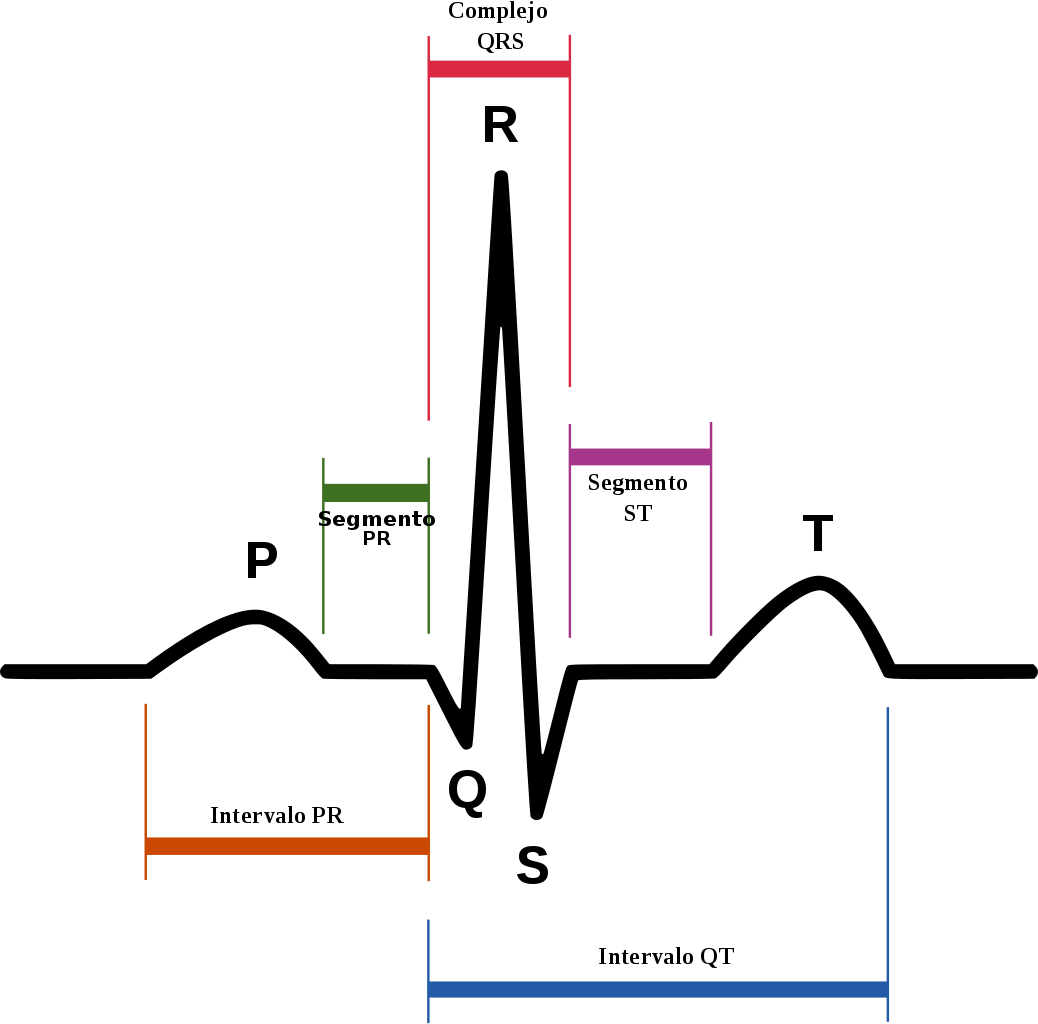
\includegraphics[width=0.5\linewidth]{Sem_1/figuras/1038px-SinusRhythmLabels-es.svg}
    	\caption{ECG con ritmo sinusal normal y las partes de este debidamente identificadas}
    	\label{fig:ECGSinusal}
    \end{figure}
    \\
    
    Como se observa en la figura \ref{fig:ECGSinusal} el ECG consta de varias ondas representativas de cada etapa de un latido cardíaco, estas son: \\

	
	\begin{itemize}
		\item \textbf{Onda P}: registra la despolarización auricular.
		\item \textbf{Complejo QRS}: Es la despolarización ventricular.
		\item \textbf{Onda T}: representa la repolarización ventricular.
	\end{itemize}
	
	Hoy en día el electrocardiograma es un estándar y uno de los primeros exámenes que se le hacen a los pacientes enfermos al ingresar a un centro clínico, este es registrado en un formato especialmente adaptado (tiras de papel milimetrado), estos no suelen durar más de 30 segundos. También puede ser registrada y visualizada de manera continua en un monitor similar a una pantalla de televisión, que suele ser una opción utilizada fundamentalmente en unidades de transporte sanitario medicalizadas y en unidades coronarias o de cuidados intensivos. \\
	\\
	Para intentar comprender los principios básicos que explican las oscilaciones en las líneas del ECG conviene conocer, si bien de forma somera, los fundamentos por los cuales se produce el movimiento del corazón, generado a través de microcorrientes eléctricas. De ellos es responsable el sistema de conducción eléctrica del corazón.
	
	\subsection{El sistema de conducción}
	Los impulsos eléctricos en el corazón se conducen mediante un tejido especializado al que se le denomina como sistema de conducción, este se puede describir como una intrincada red de cables a través de los cuales, y de un manera organizada, se realiza la transmisión de las microcorrientes eléctricas que generas el movimiento del corazón. La representación gráfica de estos impulsos (de estas microcorrientes) es el ECG. \\
	En el corazón normal, la frecuencia cardíaca debe ajustarse a las necesidades concretas que en un determinado momento se precisen (no tenemos las mismas pulsaciones durante el sueño que después de subir cuatro pisos). Por otro lado, las diferentes cámaras (aurículas y ventrículos) deben tener un movimiento sincronizado para que el latido cardíaco resulte eficaz. La sincronía del latido cardíaco, así como la fuerza en la contracción del corazón, se encuentran reguladas, entre otros factores, por el sistema de conducción, que consta de los siguientes elementos: 
	\begin{itemize}
		\item Nodo sinoauricular (nodo SA).
		\item Nodo auriculoventricular (nodo AV).
		\item Sistema de His-Purkinje.
	\end{itemize}
	
	\subsubsection*{El nodo sinoauricular (nodo SA)} 
	Está situado en el surco terminal entre la unión lateral de la vena cava superior con la aurícula derecha. Tiene una forma de huso con una cola larga dirigida hacia abajo por el surco terminal y en dirección del orificio de la vena cava inferior, está irrigado por la arteria nodal, rama de la arteria coronaria derecha en el $55\%$ de las veces y el resto por una rama de la arteria circunfleja. La conducción del impulso generado en el nodo, y que llega al nódulo auriculoventricular, se produce a través del músculo miocárdico auricular que por su disposición geométrica favorece la conducción preferencial \cite{fbbva}. 
	\subsubsection*{El nodo auriculoventricular (nodo AV)}
	Está localizado en el componente auricular del tabique auriculoventricular muscular, se halla subendocárdico y a la altura del vértice del triángulo delineado por el tendón de Todaro y en la inserción de la valva septal de la válvula tricúspide, estructuras que se unen en el cuerpo fibroso central. Aquí el nodo se continúa como el fascículo auriculoventricular que penetra el cuerpo fibroso y alcanza la cresta del tabique interventricular muscular debajo del septo membranoso y se bifurca en una rama derecha e izquierda. La rama derecha con un fascículo redondeado que hacia adelante se continúa hasta la región apical, penetra en la trabécula septomarginal y alcanza la pared ventricular y al musculo papilar anterior. Sus fibras forman el plexo subendocárdico de Purkinje en los músculos papilares y la pared del ventrículo derecho. Su tamaño es la mitad que el del nodo SA. Durante el paso por el nodo AV, la onda de activación eléctrica sufre una pausa de aproximadamente una décima de segundo, permitiendo así que las aurículas se contraigan y vacíen su contenido de sangre en los ventrículos antes de producirse la propia contracción ventricular. El nodo AV ejercería de esta forma un \textit{efecto embudo} en la canalización de los impulsos eléctricos en su viaje desde las aurículas a los ventrículos \cite{fbbva}.
	\subsubsection{Sistema de His-Purkinje}
	Después de atravesar el nodo AV, el impulso cardíaco se propaga por el haz de His y sus ramas ---una serie de fibras especializadas en la conducción eléctrica que discurren de arriba hacia abajo a lo largo del tabique interventricular; dicho haz de His de divide, después de un tronco común, en dos ramas, izquierda y derecha---. Cuando se emplea la expresión \textit{bloqueo de rama izquierda o bloqueo de rama derecha} se hace referencia a la interrupción de la transmisión de los impulsos eléctricos en el corazón en este nivel. Después de atravesar el haz de His, el impulso eléctrico se distribuye por toda la masa ventricular gracias a una red de microfibrillas denominadas fibras de Purkinje; se produce entonces la contracción (y consiguiente expulsión de la sangre) de ambos ventrículos \cite{fbbva}.
	\begin{figure}[h]
		\centering
		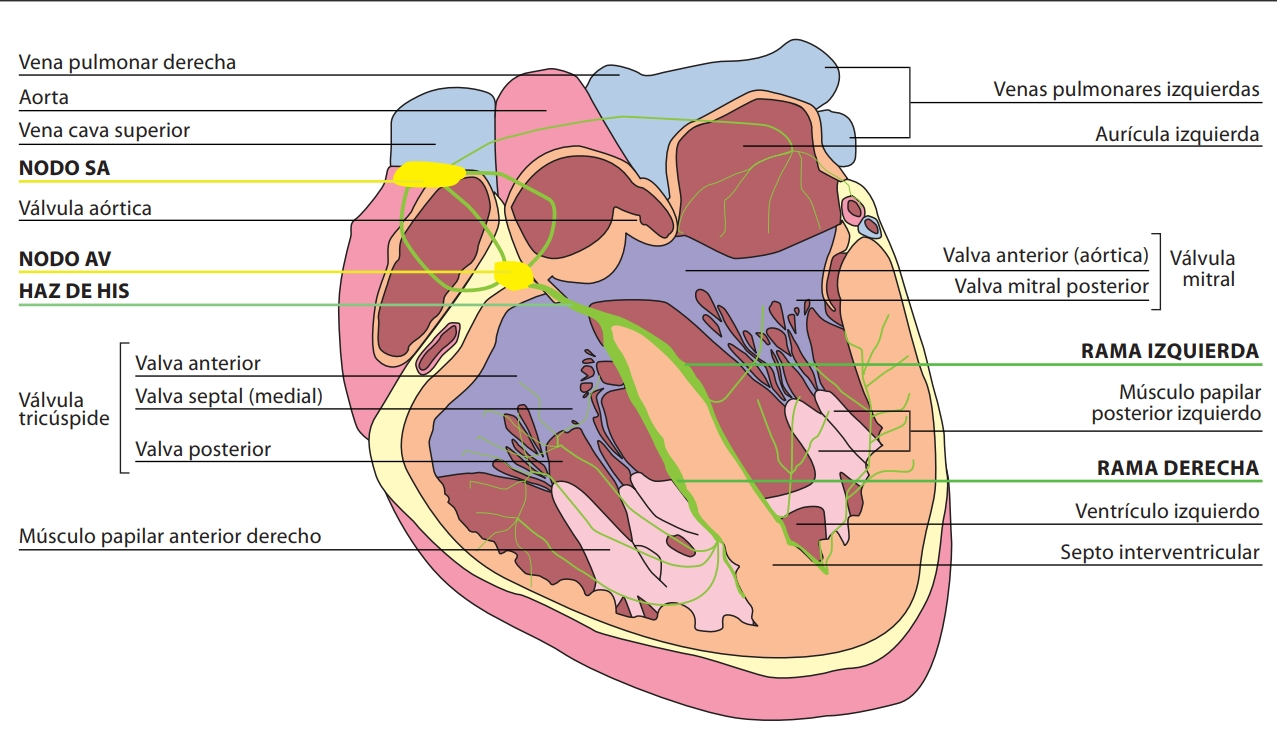
\includegraphics[width=0.95\linewidth]{Sem_1/figuras/Sistema_de_conduccion_corazon.jpeg}
		\caption{Sistema de conducción del corazón \cite{fbbva}.}
		\label{fig:sis_cond_heart}
	\end{figure}
	\subsubsection*{Actividad eléctrica de la célula miocárdica}
	La célula cardíaca posee, como las demás, una membrana celular que tiene en reposo una diferencia de voltaje entre sus dos lados. En condiciones normales y reposo, esta diferencia es de 90 milivoltios (mV). Debido a las propiedades intrínsecas de la célula, si esta es excitada, se desencadena una serie de cambios en la membrana que generan una corriente eléctrica que recorre la membrana celular y transmite el impulso eléctrico por los discos intercalares, que son membranas de baja resistencia eléctrica, entre las células, generando el potencial de acción. En el corazón normal este impulso se inicia en el nodo sinusal, debido a que tiene la descarga espontánea intermitente de frecuencia más alta en el corazón, gracias a las propiedades peculiares de la primera fase del potencial de acción en ese tejido. La disminución del potencial negativo de reposo despolariza la célula y luego se repolariza por la acción de mecanismos energéticos transmembrana que restablecen las concentraciones relativas de los iones, consumiendo energía (figura \ref{fig:fonocardio}) \cite{textCardi}.
	\begin{figure}[h]
		\centering
		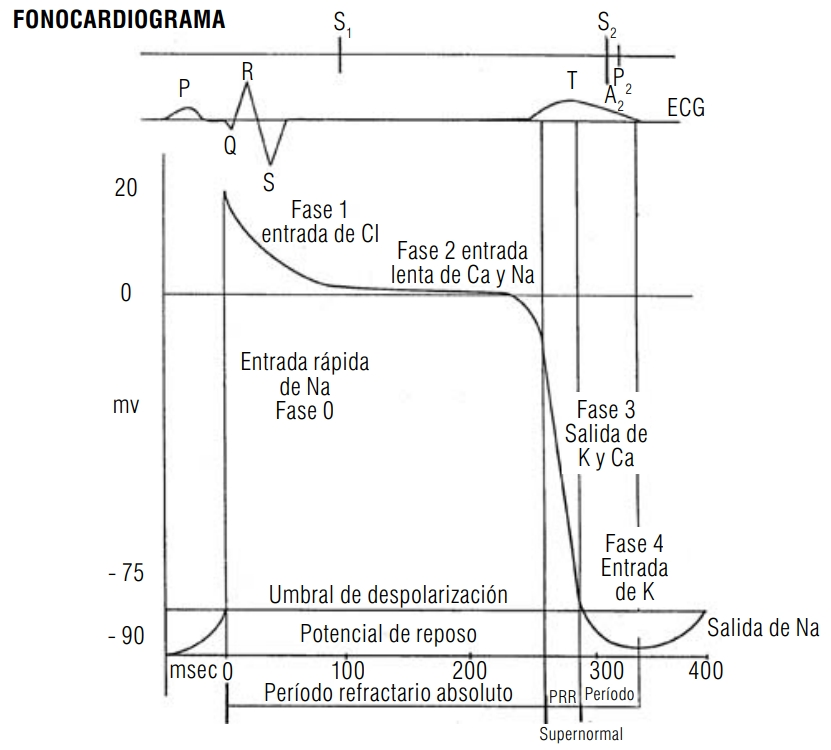
\includegraphics[width=0.8\linewidth]{Sem_1/figuras/fonocardiograma.jpeg}
		\caption{Potencial de acción-relaciones de componentes \cite{textCardi}.}
		\label{fig:fonocardio}
	\end{figure}
	
	Este potencial de acción conducido en forma adecuada es el estímulo para obtener una contracción cardíaca sincronizada. En reposo, el sodio está en el espacio extracelular en mayor concentración, al igual que el calcio, mientras que el potasio predomina en el espacio intracelular. Esto significa que la membrana tendrá una carga positiva por fuera y negativa por dentro. Al iniciarse la despolarización, ocurren cambios de la permeabilidad al sodio, lo cual permite su entrada al espacio intracelular, se invierte la carga interna, que se vuelve positiva ($+20$ mV) y la forma la fase 0 del potencial de acción. La pendiente de su ascenso regula la velocidad de conducción del tejido. Posteriormente, el cloro entra en persecución del sodio y disminuye levemente la positividad interior (fase 1). Luego baja drásticamente la permeabilidad al sodio y calcio y estos iones comienzan a disminuir su velocidad de entrada, la cual se hace básicamente a través de los canales lentos, que son voltaje dependientes y de tipo receptor de membrana que consume energía, y que inscriben una fase en meseta en el potencial de acción (Fase 2). Los canales lentos de calcio son altamente selectivos para este ion, aunque permiten la entrada también de sodio. Este mecanismo en la membrana del retículo sarcoplásmico asegura, además, que la concentración intracelular de calcio sea suficiente para los procesos contráctiles. Inmediatamente sale potasio de la célula para lograr el equilibrio de cargas eléctricas, al parecer por un súbito aumento de la permeabilidad de la membrana para este ion, disminuye la positividad y logra un potencial negativo intenso intracelular, saliendo calcio al retículo sarcoplásmico nuevamente (Fase 3). Esto repolariza la célula. Pero luego entran en acción las bombas de sodio y calcio, dependientes de ATP, que sacan Na y CA y lo intercambian por potasio, lo cual incrementa levemente el potencial intracelular (Fase 4).
	
	La velocidad de ascenso de la fase 4 es lo que regula la excitabilidad y es más pronunciado en los tejidos de excitación automática. El calcio que entra en la fase 2 es aclarado de la célula por varios mecanismos como son: las bombas de calcio dependientes de ATP, el fosfolamban, y la captación de calcio hacia el interior de la mitocondria, en un proceso que también es dependiente de energía. El potencial de acción tiene una duración variable (entre 200 y 400 ms) y durante ese período, la célula se hace total o parcialmente refractaria a una excitación adicional, al parecer por la presencia de sodio dentro de la célula. El periodo refractario absoluto ocupa las fases 0, 1, 2 y 3, es decir, mientras el sodio es aún intracelular. Una vez que el sodio comienza a salir de la célula, está parcialmente disponible para volver a entrar rápidamente, por lo que la fase 4 y la parte final de la fase 3 son el período refractario relativo. El potencial más negativo que se alcanza durante la fase 4 se atenúa en presencia de Ácidosis, hipocalemia isquemia y fibrosis y se aumenta con los medicamentos antiarrítmicos en su mayoría. Existen diferencias en la configuración del potencial de acción según el tejido analizado dentro del corazón: en las células automáticas, las fases 1 y 2 son cortas y la fase 4 es plana y en las células de conducción, la fase 0 es rápida, y la fase 2 es de mayor duración. Las fases 0 y 1 corresponden a la onda P y el complejo QRS. La fase 2 corresponde al segmento ST y la fase 3 a la onda T. La fase 4 corresponde a la diástole eléctrica. La deflexión descendente de la onda T corresponde al período refractario relativo, que tiene 2 subfases: la vulnerable que es durante la cual un estímulo de suficiente intensidad es capaz de desencadenar arritmias severas, y la subfase súper-normal, que corresponde a una hiperpolarización "muy refractaria", pues no hay potasio intracelular en cantidad abundante. La velocidad a la cual se transmite el impulso varía de acuerdo con la pendiente de la fase 0, con la altura del potencial de acción, con la duración de las fases 2 y 4. Dicha velocidad en el nodo sinusal es de $5 cm/s$, en las aurículas es de $80-100 cm/s$, en el nodo AV es de $5 cm/s$, en el haz de His es de $100 cm/s$, en las fibras de Purkinje es de $400 cm/s$ y en el músculo de $90 cm/s$
	
	Las células miocárdicas tienen varias propiedades únicas, entre ellas está la Automaticidad que no es más que la capacidad de descarga espontánea a una frecuencia fija, dependiente de la pendiente de la fase 4; La Excitabilidad es esa capacidad de respuesta al estímulo; y por último, la Conductividad que es esa capacidad de transmitir el impulso de una célula a otra.
	
\subsection{Interpretación de un electrocardiograma}

El ECG presenta como línea guía la denominada \textit{línea isoeléctrica o línea basal}, que puede identificarse fácilmente como la línea horizontal existente entre cada latido. Los latidos cardíacos quedan representados en el ECG \textit{normal} por las diferentes oscilaciones de la línea basal en forma de ángulos, segmentos, ondas e intervalos, constituyendo una imagen característica que se repite con una frecuencia regular a lo largo de la tira de papel del ECG. Como se ha comentado, entre latido y latido va discurriendo la línea base. \\
El recorrido en sentido horizontal hace referencia al \textit{tiempo} transcurrido, y la distancia en sentido vertical (amplitud) al \textit{voltaje} que se está produciendo. El papel por el que discurre el registro de la línea se encuentra milimetrado. Cada cuadrado pequeño del papel mide $1 mm$ y al observarlo con detenimiento puede comprobarse que cinco cuadrados pequeños forman un cuadrado grande, remarcado por un grosor mayor en la tira de papel de ECG. Para conocer cómo transcurren los tiempos durante la actividad del corazón, basta con recordar que cinco cuadrados grandes en sentido horizontal equivalen exactamente a un segundo. \\
En un ECG \textit{normal}, cada complejo consta de un a serie de deflexiones (ondas del ECG) que alternan con la línea basal. Realizando la lectura de izquierda a derecha, se distinguen la onda P, sel segmento P-R, el complejo QRS, el segmento ST y finalmente la onda T, véase la figura \ref{fig:ECGSinusal}. \\

\subsubsection{Onda P}

Es la primera deflexión hacia arriba que aparece en el ECG. Su forma recuerda a una mezcla entre una U y una V invertidas. Suele durar entre $80-100 ms$ y esta representa el momento en que las aurículas se están contrayendo y enviando sangre hacia los ventrículos. 

\subsubsection{Segmento P-R}

Es el tramo de la línea basal (línea isoeléctrica) que se encuentra entre el final de la onda P y la siguiente deflexión ---que puede ser hacia arriba (positiva) o hacia abajo (negativa)--- del ECG. Durante este período, las aurículas terminan de vaciarse y se produce una relativa desaceleración en la transmisión de la corriente eléctrica a través del corazón, justo antes del inicio de la contracción de los ventrículos. 

\subsubsection{Complejos QRS}

Corresponde con el momento en que los ventrículos se contraen y expulsan su contenido sanguíneo. Como su nombre indica, consta de las ondas Q, R y S. La onda Q no siempre está presente. Se identifica por ser la primera deflexión negativa presente después del segmento P-R. Toda la deflexión positiva que aparezca después del segmento P-R corresponde ya a la onda R propiamente dicha y, como se ha comentado anteriormente, el hecho de que no vaya precedida por una onda Q no es en absoluto patológico. De hecho, y siempre en relación con una ECG normal, las ondas Q deben ser de pequeño tamaño ---no mayores que un cuadrado pequeño en el papel milimetrado, tanto en longitud (duración) como en profundidad (voltaje)--- y encontrarse presentes sólo en ciertas derivaciones. La onda R es muy variable en altura, ya que puede llegar a medir desde $2 mm$ hasta $8-10 mm$ en el caso de personas jóvenes deportistas. La onda S se observa como continuación directa de la onda R y comienza a partir del punto en que esta última, en su fase decreciente, se hace negativa.\\
En conjunto, el complejo formado por las ondas Q, R y S no debe exceder en duración más de dos cuadrados pequeños. 

\subsubsection{Segmento ST}

En el trazado de la línea basal que se encuentra entre el final de la onda S y el comienzo de la onda T. Su elevación o descenso en relación con la línea basal puede significar insuficiencia en el riego del corazón, especialmente si dichas oscilaciones coinciden con sintomatología característica que pueda expresar afectación en el aporte de oxígeno al corazón. En este sentido, su valor como herramienta diagnóstica resulta insustituible.

\subsubsection{Onda T}

Se inscribe a continuación del segmento ST. Consiste en una deflexión normalmente positiva que asemeja el relieve de una montaña más o menos simétrica. Su duración suele estar entre $0,1-0,25 s$ y no debe exceder los $0,3 s$. La onda T representa el momento en que el corazón se encuentra en un período de relajación, una vez que ha expulsado la sangre que se hallaba en los ventrículos.

\subsection{Realización de un electrocardiograma}

Realizar un ECG es un procedimiento sencillo. Se necesitan un electrocardiógrafo, parches de ECG que actúan como sensores sobre la piel, comportándose como si fueran electrodos, y un sistema de cables que transmiten las microcorrientes recogidas por los parches al electrocardiógrafo, el cual se encargará de amplificarlas. El paciente se coloca boca arriba sobre una camilla. La postura ideal es completamente horizontal; en caso de no tolerar bien esta posición, la camilla podría elevarse unos treinta grados. \\
Un enfermero, un técnico o un médico le colocarán un total de 10 parches (electrodos). Se coloca uno en cada extremidad, formando así las seis derivaciones llamadas \textit{de los miembros}. Los restantes seis parches se colocan en seis puntos específicos del pecho en la denominada \textit{región precordial}, y hacen referencia a las seis derivaciones precordiales. Una derivación electrocardiográfica está constituida por la unión de dos electrodos. De esta forma, es posible conseguir un total de 12 derivaciones. Cada una permite obtener una visión electrocardiográfica diferente, representando 12 \textit{ventanas} o puntos de observación distintos. Así, una anomalía que afecta a una parte concreta del corazón puede no ser advertida desde una derivación (ventana) y sí desde otra. Esta característica confiere valor al ECG para localizar la zona del corazón que puede encontrarse dañada. Cada derivación presenta un patrón del ECG característico con el que el médico está familiarizado, pero los principios expuestos en la descripción del ECG son aplicables a todas las derivaciones. \\
Una vez que el paciente se encuentra tumbado y con los 10 cables que conectan el ECG con su parche (electrodo) correspondiente, se puede comenzar el registro del ECG, cuya duración aproximada es de 10 segundos. El registro obtenido ---gracias a la impresora que lleva incorporado el propio ECG--- constituye el ECG del paciente. \\
Es importante tener en cuenta que desde el momento en que el operador indica que va a comenzar el registro, el paciente debe moverse lo menos posible, ya que incluso el temblor muscular fino (por ejemplo, por frío o intranquilidad) puede interferir con la señal del registro, y en el caso de resultar excesivamente distorsionada será preciso repetir el ECG. Asimismo, el contacto entre los parches y la piel del enfermo debe ser lo más estrecho posible y, en este sentido, al realizar un ECG hay que evitar la utilización previa de cremas o lociones que interfieran en dicho contacto. Es frecuente que el operador tenga que emplear una gasa suavemente impregnada en alcohol, ya que la propia grasa de la piel puede interferir con la nitidez del registro, y aplicarla sobre los puntos donde serán situados los parches.\\ Éstos llevan un gel autoadhesivo cuya composición favorece la transmisión de las pequeñas corrientes eléctricas desde la piel al electrocardiógrafo. Este gel conductor tiene una caducidad relativamente temprana y ocasionalmente puede ocurrir que la señal eléctrica no pueda ser recogida por el electrocardiógrafo debido a anomalías o defectos del parche. En este caso, en el papel del ECG no aparecerá ningún tipo de señal, ninguna línea. Naturalmente, la situación queda subsanada en cuanto se desprendan los parches defectuosos y se repita el ECG utilizando los adecuados. \\
Hoy en día, un ECG puede ser realizado en cualquier sitio debido tanto a la reducción en el tamaño de los equipos como, sobre todo, a la posibilidad de disponer el electrocardiógrafos portátiles. De esta forma, el ECG llega al domicilio de pacientes que no se pueden desplazar o al lugar donde se ha producido un accidente y, naturalmente, se puede disponer de monitorización con ECG continua durante el transporte sanitario. Pese a todo, lo más frecuente es que el ECG se realice dentro del medio hospitalario o bien a nivel ambulatorio en centros de salud o consultorios médicos.

Existen otras formas de realizar un ECG aparte de la convencional en reposo. Fundamentalmente son dos: el ECG de esfuerzo que consiste en caminar en una cinta sin fin o pedalear en una bicicleta especialmente adaptada, mientas un médico valore el ECG realizado durante el ejercicio, y el Holter-ECG, en el que se registra el ECG del paciente mediante un sistema de grabación especialmente diseñado, durante un tiempo aproximado de 24 horas; posteriormente, es analizado por un \textit{software} específico y este, se utiliza principalmente para el estudio de arritmias \cite{textCardi}. 

El ECG es una prueba diagnóstica asequible, segura y sencilla de realizar, que proporciona una gran cantidad de información con relación al estado del corazón. Fundamentalmente, se utiliza para detectar trastornos del ritmo cardíaco (arritmias) y en el diagnóstico de trastornos del flujo coronario, como lo son las cardiopatías coronarias. Asimismo, el ECG es el método de elección en el diagnóstico de los bloqueos cardíacos, en los cuales la transmisión del impulso ha quedado parcial o completamente interrumpida en algún de su recorrido a través del sistema de conducción. El ECG también se utiliza, aunque en menor medida, en el diagnóstico del aumento de tamaño de las cavidades del corazón. Este hecho se observa muy frecuentemente en la hipertensión arterial, en la cual el corazón tiene que bombear contra una resistencia que se encuentra aumentada. También, algunos trastornos de los electrolitos sanguíneos, especialmente el calcio y el potasio, tienen también su reflejo en el ECG, que naturalmente su nivel exacto se obtendrá a través de un análisis de sangre, pero el ECG puede resultar orientativo en cuanto al grado de gravedad de la alteración. Finalmente, el ECG también resulta útil en el seguimiento de las enfermedades cardíacas al establecerse una comparación con los electros previos del paciente. Así, ayuda al médico a valorar el desarrollo evolutivo de una determinada patología y, en ocasiones, es de gran utilidad a la hora de establecer un tratamiento concreto o de modificar la dosis de algún medicamento que el paciente pueda estar tomando. 

Para efectuar un ECG no se precisa ninguna preparación en concreto, además que no existen riesgos en la realización de un ECG, ya que es una prueba segura y exenta de ellos. La actividad eléctrica reflejada en el papel es generada por el propio organismo, de ahí que el paciente no sienta nada durante el registro. 

\section{Conceptos específicos}

\subsection{Aprendizaje Automático}
	El aprendizaje automático se ha vuelto uno de los más importantes temas hoy en día, constantemente se busca la manera de sacar el mayor provecho de los datos que se tengan recopilados con el fin de desarrollar estrategias que ayuden a tener un nivel superior de entendimiento de estos. Con los modelos de aprendizaje automático apropiados, se tiene la habilidad de hacer predicciones precisas en el mundo real y a medida que nueva data es constantemente agregada, se asegura que los modelos continúen rindiendo eficientemente y siendo capaces de adaptarse a los problemas del mundo real. 

	El aprendizaje automático es una de las ramas de la Inteligencia Artificial (IA) que le permite a un sistema aprender de los datos que se le dan en lugar de programarle explícitamente la tarea que debe desempeñar. 
	
	El aprendizaje automático usa una variedad de algoritmos que interactivamente aprenden de los datos, para mejorar, describir datos e incluso, predecir resultados. Como estos algoritmos constantemente ingieren datos de entrenamiento, es entonces posible producir modelos más precisos basados con esta data. El aprendizaje automático engloba tantos algoritmos que es necesario agruparlos por categorías o paradigmas de aprendizaje, estos se dividen en función de la salida de los mismos.

\subsection{Análisis de Componentes Principales (PCA).}
	Los grandes conjuntos de datos están cada vez más extendidos en muchas disciplinas. Para interpretarlos, se necesitan métodos que reduzcan drásticamente su dimensionalidad de forma interpretable, de modo que se conserve la mayor parte de la información contenida en los datos. Se han desarrollado muchas técnicas con este fin, pero el análisis de componentes principales (PCA) es una de las más antiguas y utilizadas. Su idea es sencilla: reducir la dimensionalidad de un conjunto de datos conservando la mayor cantidad posible de «variabilidad», es decir, de información estadística.
	
	Esto significa que «preservar tanta variabilidad como sea posible» se traduce en encontrar nuevas variables que sean funciones lineales de las del conjunto de datos original, que maximicen sucesivamente la varianza y que no estén correlacionadas entre sí. PCA usa álgebra lineal para transformar datos a unas variables llamadas componentes principales (PC). Estas se encuentras calculando los autovectores (direcciones) y autovalores (importancia) de una matriz de covarianza. PCA selecciona los componentes principales con los autovalores más altos y proyecta los datos sobre ellos, para simplificar el conjunto de datos. Para esto se debe: \\
	\begin{enumerate}
		\item \textbf{Estandarizar los datos.} \\
		Las diferentes caracteristicas que están presentes en el conjunto de datos pueden tener diferentes unidades y escalas. Para comparar estas equitativamente, primero se debe estandarizar los datos haciendo que cada característica tenga: 
		\begin{itemize}
			\item Una media de $0$.
			\item Una desviación estándar de $1$.
		\end{itemize}
		\begin{equation}
			\label{eq:standard}
			Z = \frac{\textit{X}-\mu}{\sigma}
		\end{equation}
		donde:
		\begin{itemize}
			\item $\mu$ es la media de las caracteristicas independientes $\mu = \{\mu_1, \mu_2,\dotsb,\mu_m\}$
			\item $\sigma$ es la desviación estándar de las caracteristicas independientes $\sigma = \{\sigma_1, \sigma_2,\dotsb,\sigma_m\}$
		\end{itemize}
		\item \textbf{Calcular la matriz de covarianza.}\\
		Es necesario calcular la matriz de covarianza para ver como las caracteristicas se relacionan entre sí, si estas aumentan o disminuyen juntas. La matriz de covarianza entre dos caracteristicas $x_1$ y $x_2$ es:
		\begin{equation}
			\label{eq:covarianza}
			\operatorname{cov}(x 1, x 2)=\frac{\sum_{i=1}^n\left(x 1_i-\bar{x} 1\right)\left(x 2_i-\bar{x} 2\right)}{n-1}
		\end{equation}
		donde: 
		\begin{itemize}
			\item $\bar{x}_1$ y $\bar{x}_2$ son los valores medios de las caracteristicas $x_1$ y $x_2$.
			\item $n$ es el numero total de datos.
		\end{itemize}
		El valor de la covarianza puede ser positivo, negativo o cero.
		\item \textbf{Encontrar las componentes principales.}
		PCA identifica los \textit{nuevos ejes} donde la varianza de los datos es mayor:
		\begin{itemize}
			\item \textbf{1er Componente Principal (PC1):} La dirección donde está la mayor dispersión de los datos.
			\item \textbf{2da Componente Principal (PC2):} La siguiente mejor dirección, \textit{perpendicular a PC1} y así sucesivamente.
		\end{itemize}
		Estas direcciones vienen de los autovectores de la matriz de covarianza y su importancia es medida por los autovalores. Para una matriz $A$, un autovector $X$ (un vector no nulo) y su correspondiente autovalor $\lambda$ satisface:
		\begin{equation}
			\label{eq:autovalores}
			AX = \lambda X
		\end{equation}
		Esto significa:
		\begin{itemize}
			\item Cuando $A$ actuá sobre $X$ sólo estira o encoge $X$ por el escalar $\lambda$.
			\item La dirección de $X$ no cambia, por lo que los autovectores definen \guillemetleft direcciones estables\guillemetright \ de $A$.
		\end{itemize}
		\item \textbf{Selecciona las mejores direcciones y transforma los datos.}
		Después de calcular los autovalores y autovectores, PCA clasifica estos por la cantidad de información que ellos capturan. Entonces: 
		\begin{itemize}
			\item Selecciona los k componentes principales que capturan la mayor parte de la varianza, como el 95\%.
			\item Transforma el conjunto de datos original proyectándolo sobre los mejores componentes principales. 
		\end{itemize}
		Esto significa que se reduce el numero de caracteristicas (dimensiones) mientras se mantienen los patrones importantes que están implícitos de los datos.
	\end{enumerate}
	
	Hasta que no se generalizó el uso de ordenadores electrónicos, que fue posible utilizarlo con conjuntos de datos que no fueran trivialmente pequeños. Desde entonces, su uso se ha multiplicado y se han desarrollado numerosas variantes en muchas disciplinas diferentes.
	
%	La definición formal de PCA, en un contexto estándar, junto con una derivación que muestra que puede obtenerse como la solución a un problema de auto-valores y auto-vectores o, alternativamente, a partir de la descomposición del valor singular (SVD) de la matriz (centrada) de datos. El PCA puede basarse en la matriz de covarianzas o en la matriz de correlaciones. Se discutirá la elección entre estos análisis. En ambos casos, las nuevas variables (las PC) dependen del conjunto de datos, en lugar de ser funciones de base predefinidas, por lo que son adaptativas en sentido amplio. Los principales usos del PCA son descriptivos y no inferenciales.\cite{Joliiffe16}\\

\subsection{Incrustación de vecinos estocásticos distribuidos en t (t-SNE)}
	 La incrustación de vecinos estocásticos comienza convirtiendo las distancias Euclidianas altas dimensionales entre los puntos de datos en probabilidades condicionales que representan similaridades. Según van der Maaten y Hinton: "La similaridad entre el punto $x_i$ $x_j$ es proporcional a la probabilidad condicional $p_{i\mid j}$ de que $x_i$ escoja a $x_j$ como su vecino si los vecinos se eligieran en proporción a su densidad de probabilidad bajo una gaussiana centrada en $x_i$". Para puntos de datos cercanos, $p_{i\mid j}$ es relativamente alta, mientras que para puntos de datos muy separados, $p_{i\mid j}$ será casi infinitesimal (para valores razonables de la varianza en la gaussiana, $\sigma_i$). Matemáticamente, la probabilidad condicional $p_{i\mid j}$ es dada por: 
	 \begin{equation}
	 	\label{eq:prob_cond}
	 	p_{j \mid i}=\frac{\exp \left(-\left\|x_i-x_j\right\|^2 / 2 \sigma_i^2\right)}{\sum_{k \neq i} \exp \left(-\left\|x_i-x_k\right\|^2 / 2 \sigma_i^2\right)},
	 \end{equation}
	donde $\sigma_i$ es la varianza de la Gaussiana que está centrada en el punto $x_i$. Debido a que estamos interesados en modelar las similaridades entre pares, se establece $p_{i\mid j} = 0$. Observe que el denominador anterior garantiza $\sum_j p_{j \mid i}=1$ para todas las $i$. Para las contrapartes de baja dimensionalidad $y_i$ y $y_j$ de los puntos altos dimensionales $x_i$ y $x_j$, es posible calcular una probabilidad condicional similar, la cual se denotará por $q_{j \mid i}$. De ahí que, se modela la similaridad de un punto cartográfico $y_j$ con el punto cartográfico $y_i$ por:
	\begin{equation}
		\label{eq:prob_cond_q}
		q_{j \mid i}=\frac{\exp \left(-\left\|y_i-y_j\right\|^2\right)}{\sum_{k \neq i} \exp \left(-\left\|y_i-y_k\right\|^2\right)}
	\end{equation}
	Al igual que en el caso anterior, como sólo se está interesado en el modelado de las similaridades en cada par de puntos, se establece $q_{i \mid i}=0$.
	Las probabilidades condicionales $q_{i \mid i}$ y $p_{i \mid i}$ serán iguales siempre y cuando los puntos cartográficos $y_i$ y $y_j$ modelen correctamente la similaridad entre los puntos alto dimensiones $x_i$ y $x_j$.\\ En este caso, se utiliza una distribución t de Student de colas gruesas para medir las similitudes entre puntos cartográficos de baja dimensión, con el fin de permitir que los objetos se modelen muy separados entre si. 
	Se busca una representación bajo dimensional de los datos que minimice la disparidad entre $q_{i \mid i}$ y $p_{i \mid i}$, para lograr esto, se usa como medida de fidelidad entre $q_{i \mid i}$ y $p_{i \mid i}$, la divergencia de Kullback-Leibler. Haciendo uso del método de gradiente descendiente t-SNE, minimiza la suma de las divergencias de Kullback-Leibler sobre todos los puntos, teniendo una función de costo dada por: 
	\begin{equation}
		\label{eq:func_costo}
		C = \sum_i KL(P_i\|Q_i)=\sum_i\sum_j p_{j\mid i}\log\frac{p_{j\mid i}}{q_{j\mid i}},
	\end{equation}
	en la cual $P_i$ representa la distribución de probabilidad condicional sobre todos los puntos de datos, dado el punto $x_i$, y $Q_i$ representa la distribución de probabilidad condicional sobre todos los puntos de datos, dado el punto $y_i$ y es el resultado de esta optimización, un mapa que refleja las similitudes entre las entradas de alta dimensión.
%	Aca estoy dudoso si tambien hablar sobre el perplexity y todo lo que viene despues de eso
	
\subsection{K-medios (k-means)}

	Los problemas de agrupamiento aparecen en diferentes aplicaciones, como reconocimiento y clasificación de patrones, de acá surge en la búsqueda de algoritmos que permitan visualizar los datos en forma de grupos o \textit{clusters}\footnote{Cúmulo, grupo o racimo}. La noción de lo que constituye un buen clúster depende de su aplicación y de la aproximación con la que se llega a este. La mayoría de las formulaciones de los métodos de agrupamiento, están basadas en minimizar una función objetiva y quizás el algoritmo más usado y estudiado es \textit{k-means}. Dado un conjunto de puntos $\mathbf{x}=\{x_1,x_2,\dotsb,x_n\}$ en un espacio real \textit{d}-dimensional, $\mathbf{R}^d$, y un entero \textit{k} ($k \leq n$), el problema es entonces, determinar un conjunto de \textit{k} puntos en $\mathbf{R}^d$, llamados \textit{centroides} $S_k$, que minimicen la \textit{inercia} o la suma de cuadrados de cada grupo (WCSS, por sus siglas en inglés) desde para punto de los datos a su centroide más cercano, esto es: 
	\begin{equation}
		\label{eq:min_k_means}
		\underset{\mathbf{S}}{\arg \min } \sum_{i=1}^k \sum_{\mathbf{x}_j \in S_i}\left\|\mathbf{x}_j-\boldsymbol{\mu}_i\right\|^2
	\end{equation}
	Se puede decir que la \textit{inercia} es una medida de que tal coherentes son los clusters internamente, esto lleva a que se sufran de algunos inconvenientes:
	\begin{itemize}
		\item La \textit{inercia} no es una métrica normalizada, por lo que en espacios muy alto dimensionales, las distancias Euclidianas tienden a volverse infladas (a esto se le llama "maldición de la dimensionalidad"). Es por esto que aplicar algoritmos de reducción de dimensionalidad como PCA previo a k-means, puede agilizar y aliviar el consumo computacional.
		\item k-means responde ineficientemente a clusters alargados o grupos con formas irregulares, debido a que la \textit{inercia} presume que los clusters son convexos e isotrópicos.
	\end{itemize}
	El algoritmo estándar de k-means, fue propuesto inicialmente por Stuart Lloyd en 1957, quien lo propuso como una técnica para modulación por impulsos codificados, sin embargo este no fue publicado hasta 1982, es por esto que a este algoritmo también se le conoce como algoritmo de Lloyd, sobre todo en la comunidad informática. \\
	
	\textbf{Algoritmo k-means (basado en MacKay, 2003 \cite{mackay03}):}
	\begin{enumerate}
		\item \textbf{Inicialización:} 
		Se eligen los $k$ centroides $\left\{\mathbf{m}^{(k)}\right\}$ aleatoriamente.
		\item \textbf{Paso de asignación:}
		Cada punto $\mathbf{x}^{(n)}$ se asigna al centroide más cercano. La asignación se denota como $\hat{k}^{(n)}$:
		\begin{equation}
			\label{eq:k_mean_asig}
			\hat{k}^{(n)}=\underset{k}{\operatorname{argmin}}\left\{d\left(\mathbf{m}^{(k)}, \mathbf{x}^{(n)}\right)\right\}
		\end{equation}
		Una representación alternativa y equivalente de esta asignación de puntos a los conglomerados viene dada por las \textit{responsabilidades}, que son variables indicadoras $r_k^{(n)}$. En el paso de asignación, establecemos $r_k^{(n)}$ en uno si la media $k$ es la media más cercana al punto de datos $\mathbf{x^{(n)}}$; de lo contrario $r_k^{(n)}$ es cero.
		\begin{equation}
			\label{eq:cond_rk}
			r_k^{(n)}=\left\{\begin{array}{lll}
				1 & \text { si } & \hat{k}^{(n)}=k \\
				0 & \text { si } & \hat{k}^{(n)} \neq k
			\end{array}\right.
		\end{equation}
		\item \textbf{Paso de actualización:}
		Los parámetros del modelo, las medias, se ajustan para que coincidan con las medias muestrales de los puntos de datos de los que son responsables.
		\begin{equation}
			\label{eq:media_muestral}
			\mathbf{m}^{(k)}=\frac{\sum_n r_k^{(n)} \mathbf{x}^{(n)}}{R^{(k)}}
		\end{equation}
		donde $R^{(k)}$ es la \textit{responsabilidad} total de la media $k$.
		\begin{equation}
			\label{eq:rk}
			R^{(k)}=\sum_n r_k^{(n)}
		\end{equation}
		\item \textbf{Se repiten los pasos de asignación y actualización} hasta que no hayan cambios en la asignación.
	\end{enumerate}
	
\subsection{Redes Neuronales}
	Una red neuronal artificial es un programa que intenta imitar la manera en que un cerebro humano es capaz de abordar ciertos problemas, esta usa capas interconectadas de unidades, llamadas perceptrones, siendo capaces de aprender e inferir reglas o relaciones basados en la data observada, dicha red adquiere los conocimientos mediante un proceso de entrenamiento y aprendizaje, donde almacena \textit{conocimiento} este utilizando intensidades de conexión interperceptrónica. 
	
	Estos métodos pueden utilizarse como método alternativo en análisis y predicciones. Al estudio de estas redes se le conoce como Aprendizaje Profundo y su uso esta siendo elevado hoy en día en numerosas aplicaciones, desde manejo autónomo de vehículos hasta en aplicaciones de imágenes medicas.\\ Su funcionamiento es del tipo «caja negra», es decir, estos modelos no requieren información detallada del sistema ya que aprenden de la relación entre los parámetros de entrada, similar a una regresión no lineal, pero con mucha más potencia que una de estas, manejando sistemas grandes y complejos con muchos parámetros interrelacionados.
	
	La red neuronal más simple es aquella compuesta por una sola neuronal, es decir, que el modelo matemático más sencillo es un perceptrón, este, según Frank Rosenblatt \cite{perceptron} es "la unidad básica de inferencia en forma de discriminador lineal, a partir de lo cual se desarrolla un algoritmo capaz de generar un criterio para seleccionar un subgrupo a partir de un grupo de componentes más grande."
	
	Este toma un vector de valores reales como entrada, calcula una combinación lineal de estas, después da una salida de 1 si el resultado es mayor que algún umbral, de lo contrario y de acuerdo a la función de activación que se use, la salida tendrá como resultado 0 o cualquier otro valor diferente de 1. Más precisamente, dadas las entradas $x_1$ hasta $x_n$, la salida $o(x_1,\dotsb,x_n)$ calculada por el perceptrón es: 
	\begin{equation}
		\label{eq:percept}
		o(x_1,\dotsb,x_n) = \left\{\begin{array}{lll}
			1 & \text { si } w_0 + w_1x_1 + w_2x_2 + \dotsb + w_nx_n > 0 \\
			0 & \text { en otro caso } 
		\end{array}\right.
	\end{equation}
	donde cada $w_i$ es una constante real conocida como «pesos», estos determinan la contribución de la entrada $x_i$ en la salida del perceptrón.
	\begin{figure}[h]
		\centering
		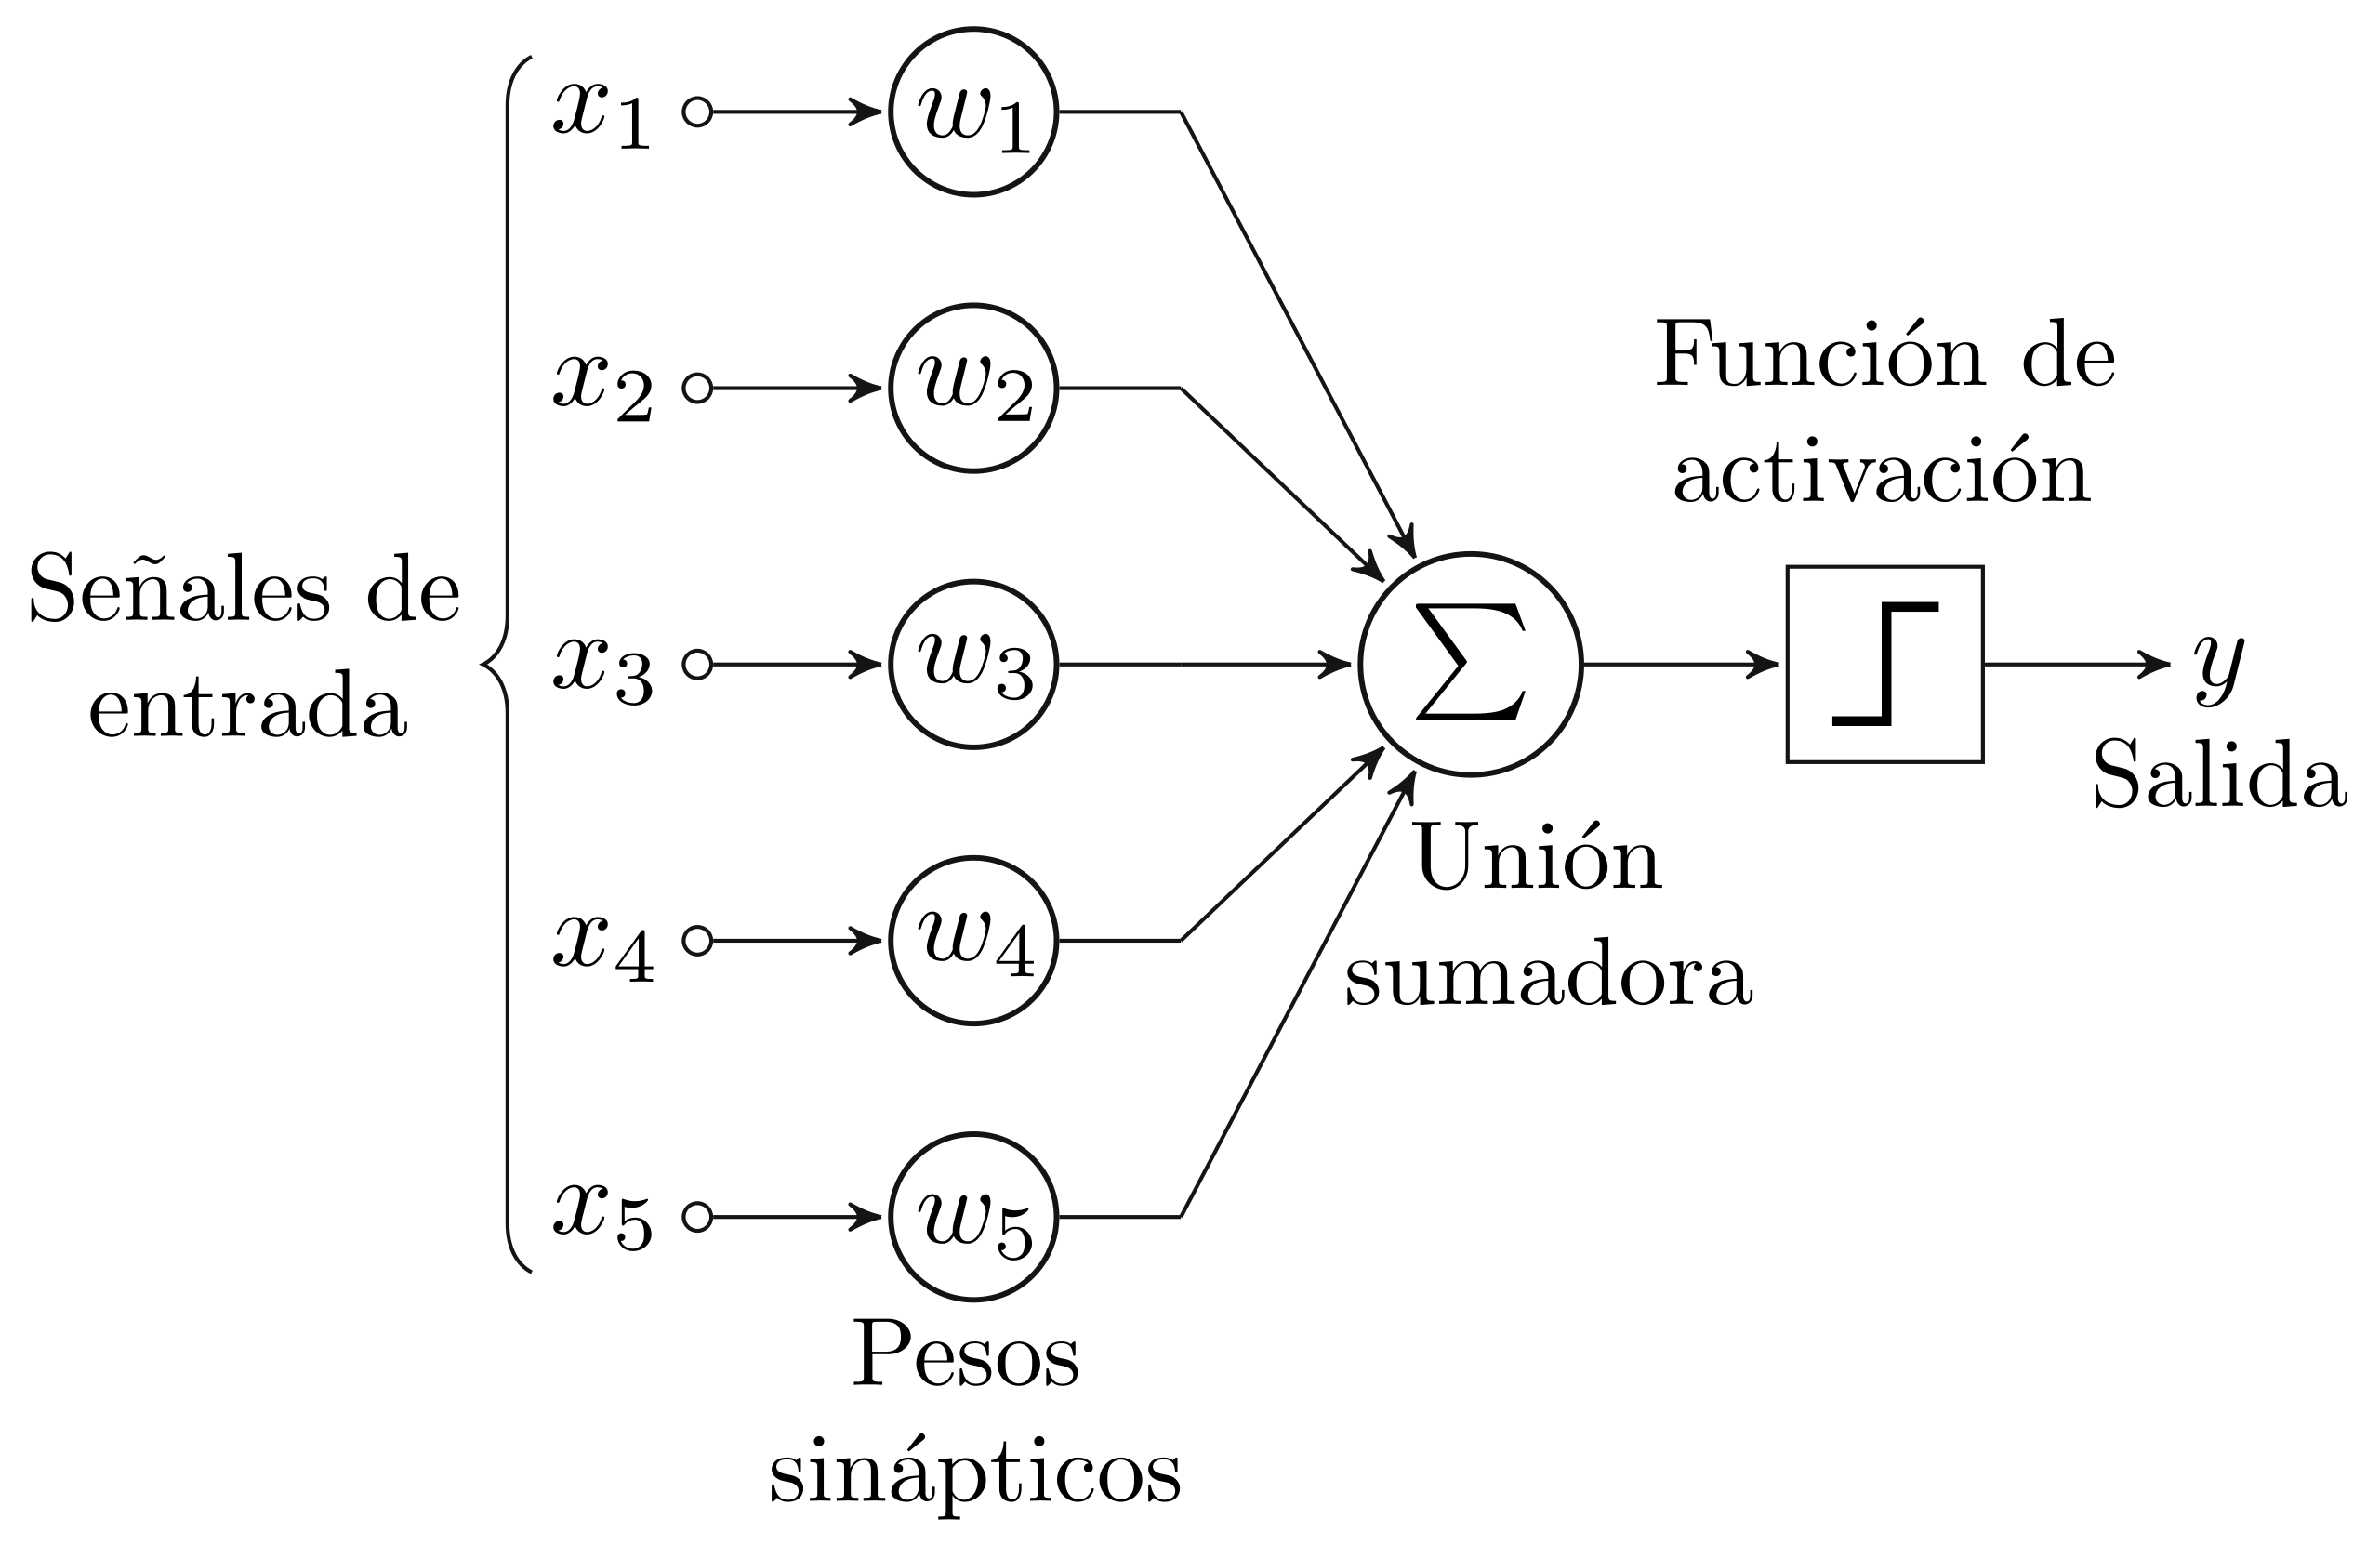
\includegraphics[width=0.8\linewidth]{Sem_1/figuras/Perceptron}
		\caption{Diagrama de un perceptrón con cinco señales de entrada \cite{imaPercep}.}
%		\label{fig:}
	\end{figure}
	
	
	


%\part{Segundo seminario}
\chapter{Marco experimental}

...

\chapter{Resultados}

...

\part{Conclusiones}
\chapter{Conclusiones}

...

% Bibliografía
\bibliographystyle{ieeetr}
\bibliography{bibliografia.bib} 

\end{document}
